\documentclass[11pt]{article} %Tamaño de la letra

%Paquetes esenciales
\usepackage[spanish]{babel}
\usepackage[utf8]{inputenc}
\usepackage[T1]{fontenc}
\usepackage{float}
%Fuente arial
\usepackage{helvet}
\renewcommand{\familydefault}{\sfdefault}

%Hipervinculos y citas
\usepackage{csquotes}
\usepackage[backend=biber, style=apa, sortlocale=es]{biblatex} % <-- CORREGIDO
\usepackage{hyperref} % <-- CORREGIDO: estaba mal escrito como 'hyperrref'
\usepackage{url}
%Graficos y color
\usepackage{graphicx} % Required for inserting images
\usepackage{xcolor}
\usepackage{tikz}
\usetikzlibrary{positioning}


%Margenes y espacio
\usepackage[a4paper, left = 2cm, right = 1cm, top=2cm,bottom=2cm]{geometry}
\usepackage{setspace}
\linespread{1.0} %Espacio
\usepackage{setspace}


%Esto cambia el color del fondo
\pagecolor{gray!20} %Cambia este color de las paginas
\color{black} %Cambia el color del texto


%Bibilografia
\addbibresource{referencias.bib}
\begin{document}


% PORTADA
\begin{titlepage}
    \thispagestyle{empty}
    \begin{spacing}{1.5}
    \begin{center}
        
\includegraphics[width=0.2\textwidth]{Images/LogoUNA.svg.png} \\[30pt]
        {\Large \textbf{Universidad Nacional de Costa Rica}} \\[20pt] 
        {\Large Escuela de Informática} \\[20pt]
        {\Large \textbf{Redes Neuronales de Grafos (GNNs)}} \\[20pt]
        {\Large Curso: Estructuras Discretas} \\[20pt]
        {\Large \textbf{Estudiantes a cargo de la investigación:}} \\[10pt]
        {\large Sebastián Garro Granados \\ Joel Brenes Vargas \\ Santiago Jesús Hernández Chaves \\ Efraín Ignacio Retana Segura} \\[20pt]
        {\Large \textbf{Profesor a cargo del curso:}} \\[15pt]
        {\large Carlos Loria Saenz} \\[120pt]
        {\Large \textbf{Fecha:}} \\[15pt]
        {\large 17 de abril de 2025}
    \end{center}
    \end{spacing}
\end{titlepage}

% RESUMEN
\newpage
\thispagestyle{empty}
{\large \textbf{Resumen}}
\vspace{5pt}

En este trabajo se realiza la investigacion acerca de las redes neuronales de grafos (GNNs) donde se abordara la importancia, sus conceptos más importantes y como nosotros en el curso de estrucutras discretas podemos implementarlo con nuestro conocimiento adquirido en esta investigacion. Se van a desarrollar diferentes ejemplos en python, donde utilizaremos bibliotecas especializadas para implementar un GCN basico, este con el objetivo de poder ver la clasificacion de nodos en un grafo y se complementará con analisis empiricos. Además de esto, los estudiantes se dan de aprovechamiento las herramientas recomendadas por el profesor las cuales son: Github(Repositorio de pruebas), Overleaf(Documentacion) y el uso de editor de texto y compilador para crear las pruebas de GCNs en python. Este trabajo busca que el lector consiga una mejor comprension al mundo de las redes neuronales de grafos por medio de la introduccion en el documento y viendo las pruebas que se harán sobre esta. %Si quieren agregan más cosas



\newpage
\thispagestyle{empty}
{\large \textbf{Palabras claves}}
\vspace{5pt}
\newpage
\thispagestyle{empty}
{\large \textbf{Índice}}
\vspace{5pt}

\newpage
\thispagestyle{empty}
{\large \textbf{Índice de Tablas y Figuras}}
\vspace{5pt}

\newpage
\thispagestyle{empty}
{\large \textbf{Introducción}}
\vspace{5pt}
parte de garro
\newpage
\thispagestyle{empty}
{\large \textbf{Conceptos de Grafos y sus Aplicaciones}}
\vspace{5pt}
parte de garro
\newpage
\thispagestyle{empty}
{\large \textbf{Conceptos Básicos de ML usando Redes Neuronales (NNs)}} \vspace{10pt}

\textbf{a.Nociones de Machine Learning (ML)}
\vspace{5pt}

\textbf{i. Definición} 
\vspace{3pt}
\\[1pt]
El \textit{Machine Learning} (ML) es una rama o campo de la inteligencia artificial (IA) que se enfoca en el desarrollo de algoritmos capaces de aprender a partir de datos. En el pasado donde el programador tenia que escrbir explicitamente parte por parte cada regla del sistema, el \textit{machine learning} puede permitir que las computadoras identifiquen automáticamente patrones y relaciones en los datos sin tener que tener una intervención directa por el programador. Así, sea cualquier modelo puede tomar decisiones propias o generar predicciones sobre nuevos datos, basándose en lo aprendido durante en el entrenamiento de este. \\[3pt]
Basado en lo anterior mencionado, el \textit{machine learning} no sigue reglas predifinidas, los algoritmos ML analizan subconjuntos de datos para construir modelos matemáticos que representen con precisión las relaciones entre variables, incluso si estas combinaciones no son evidentes o no pueden derivarse directamente de principios lógicos.

\vspace{8pt}
\textbf{ii. Features y Datasets}\vspace{2pt}
\begin{itemize}
    \item \textbf{Features}: Los features (o atributos en español) son las variables que describen cada ejemplo y que el modelo utiliza como entrada para aprender. 
    Pueden proceder directamente de los datos originales (por ejemplo, edad, temperatura) o derivarse mediante \textit{feature engineering}, que —según la página de Google for Developers\footnote{\url{https://developers.google.com/machine-learning/glossary\#f}}— hace mención de que su significado es crear una versión más optimizada de estos features agarrándolos de su forma cruda o \textit{raw}, dicho en inglés.
\end{itemize}

\begin{figure}[H]
    \centering
    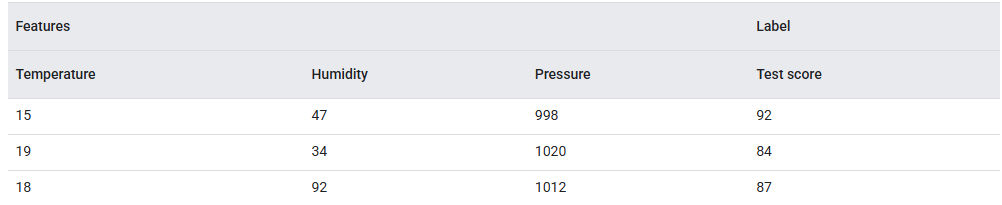
\includegraphics[width=0.8\textwidth]{Images/Imagen Proyecto.PNG}
    \caption{Ejemplo de feature simple derivado de datos crudos.}
    \label{fig:feature-simple}
\end{figure}

\begin{itemize}
    \item \textbf{Dataset}: un \textit{dataset} es la colección organizada de ejemplos sobre los que entrenamos y evaluamos el modelo. Muchos datasets se representan en tablas (por ejemplo, CSV o DataFrames), donde cada fila es un ejemplo y cada columna es un \textit{feature} o una etiqueta(\textit{label}). También pueden provenir de otros formatos como archivos de logs o protocolos binarios. Es importante para el \textit{machine learning} (ML) dividir el \textit{dataset} en subconjuntos de entrenamiento, validación y prueba para garantizar que el modelo generalice correctamente datos nuevos.
\end{itemize}

\begin{figure}[H]
    \centering
    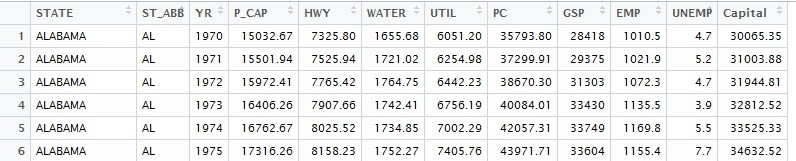
\includegraphics[width=1\textwidth]{Images/ejemplo csv2.jpg}
    \caption{Ejemplo dataset usando CSV.}
    \label{fig:Dataset-CSV}
\end{figure}
\vspace{8pt}
\textbf{iii. Entrenamiento} \\[3pt]
Es el proceso en el cual un modelo ajusta sus parámetros internos -principalmente los pesos de sus conexiones- con el objetivo de minimizar un error o función de perdida. Este proceso requiere de una base de datos etiquetada (en el caso de aprendizaje supervisada) y un algoritmo de optimización, siendo el más común \textit{descenso por el gradiente} (\textit{gradient descent}).\\[1pt]
Durante el entrenamiento, el modelo realiza predicciones sobre los datos de entrada y compara a sus resultados con las salidas reales. Con base en esa comparación, se calcula el error y se utiliza una técnica llamada \textbf{retropropagación del error} 
(\textit{backpropagation}) para distribuir este error hacia atrás a través de las capas de la red. Este mecanismo permite que cada peso se ajuste de forma proporcional al impacto que tuvo el error final. Este mismo esquema se adapta al entrenamiento de las redes neuronales de grafos (GNNs), con la diferencia de que los datos se representan como grafos, y el modelo aprende no solo de los atributos de cada nodo, sino también de su estructura y conexiones.
\begin{figure}[H]
    \centering
    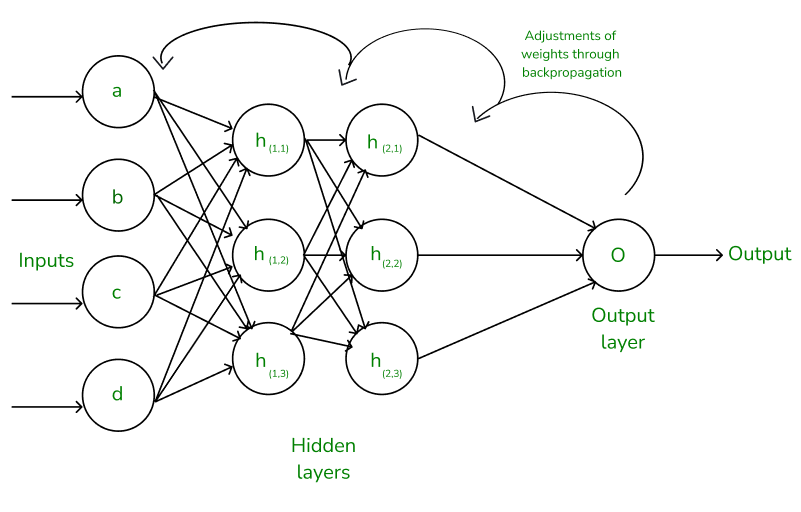
\includegraphics[width = 0.6\textwidth]{Images/Frame-13.png}
    \caption{Diagrama ilustrativo del proceso de entrenamiento y retropropagación.}
    \label{fig:Backpropagaion}
\end{figure}
\vspace{8pt}
\textbf{iv. Tipos de Aprendizaje} \\[3pt]
El \textit{Machine Learning} (ML) comprende un conjunto de técnicas y algoritmos que permiten a las máquinas aprender de los datos y realizar predicciones o tomar deciones sin estar explícitamente programadas para cada tarea, una de las distinciones fundamentales dentro del ML se basa en el tipo de datos disponibles durante el entrenamiento, especificamente en si esos datos incluyen o no etiquetas o resultados esperados. De esta forma, se clasifican los enfoques de aprendizaje en cuatros categorías principales: \textbf{supervisado}, \textbf{no supervisado}, \textbf{semisupervisado} y \textbf{por refuerzo}. Cada uno de estos métodos responde a diferentes necesidades, en esta investigación se usarán las 2 primeras, \textbf{supervisado} y \textbf{no supervisado}.
\begin{itemize}
    \item \textbf{Aprendizaje Supervisado}: Este tipo de aprendizaje se basa en un conjunto de datos etiquetado, en el que cada instancia contiene características (\textit{features}) y un resultado conocido (\textit{target}). El objetivo es que el modelo aprenda una función de mapeo $f(x) = y$, $x$ representa las entradas y $y$ la salida esperada. Para dar un ejemplo, pensemos en una empresa inmobiliaria que busca predecir el precio de una casa según su número de habitaciones, area en metros cuadrados y ubicación puede utilizar aprendizaje supervisado entrenando un modelo con ejemplos historicos de ventas. El conjunto de datos se divide usualmente en subconjuntos de entrenamiento, validación y prueba, para ajustar, afinar y evualuar el modelo, respectivamente. Las tareas tipicas en este enfoque incluyen:
    \begin{itemize}
    \item\textbf{Regresión}: predicción de valores numéricos continuos (por ejemplo, precios de viviendas).
    \item\textbf{Clasificación}: predicción de categorias discretas (por ejemplo, rango de precios como (0-125k), (125-250k), etc.).    
    \end{itemize}
    \item \textbf{No Supervisado}: A diferencia del aprendizaje supervisado, este enfoque no cuenta con etiquetas o salidas conocidas asociadas a los datos. Es decir, el modelo no tiene una \textquotedblleft respuesta correcta\textquotedblright~que pueda utilizar como guia durante el entrenamiento. En su lugar, debe analizar los datos para identificar patrones subyacentes,estructuras o agrupaciones naturales presentes en ellos. El objetivo es encontrar representaciones útiles de los datos que permiten descubrir relaciones desconocidos o inferir características relevantes sin intervención humana directa. \\[2pt]
    Este tipo de aprendizaje es especialmente útil en contextos donde obtener etiquetas es costoso y lento. En muchos casos de la vida real usando este metodo, como grandes bases de datos de clientes, imágenes, secuencias genéticas o registros médicos, se dispone de gran cantidad de informacíón sin clasificar, por lo que los algoritmos no supervisados resultan clave para el análisis exploratiorio y la extración automatica de conocimiento. \\[2pt]
    Las tareas más comunes dentro del aprendizaje no supervisado son:
    \begin{itemize}
        \item \textbf{Clustering (agrupamiento)}: agrupación de datos similares en clústeres basándose en sus características. Por ejemplo un algoritmo podría identificar subconjuntos de viviendas similares sin haber sido informado de categorías específicas.
        \item\textbf{Asociación}: descubrimiento de reglas o correlaciones frecuentes entre características. Útil para entender concurrencias comunes entre variables.
        \item\textbf{Detección de anomalías}: identificacíon de instancias atípicas o fuera de lo común, como precios de vivienda inusualmente altos en un vecindario.
    \end{itemize}
    Este tipo de aprendizaje es valioso cuando etiquetar datos resulta cosotoso o inviable, permitiendo extraer conocimiento directamente de la estructura de los datos.
\end{itemize}
\begin{figure}[H]
\centering
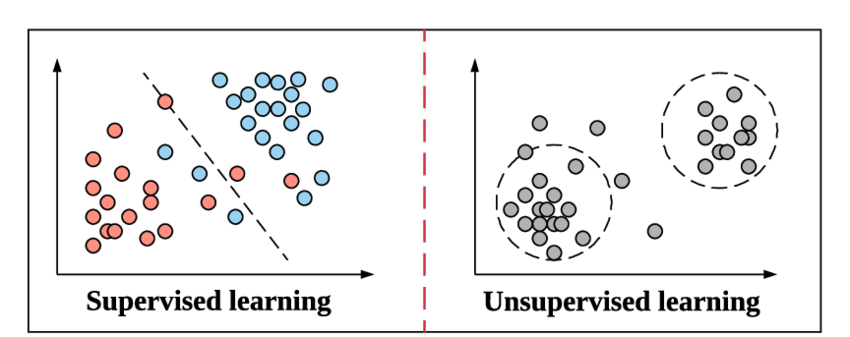
\includegraphics[width=0.7\textwidth]{Images/Examples-of-Supervised-Learning-Linear-Regression-and-Unsupervised-Learning.png}
\caption{Ejemplo gráfico comparativo de algoritmos de aprendizaje supervisado y no supervisado.}
\label{fig:aprendizaje-supervisado-no-supervisado}
\vspace{2mm}
\small\textit{Nota:} En la parte izquierda (aprendizaje supervisado), la linea discontinua representa una frontera de decisión aprendida a partir de datos etiquetados. En cambio, el gráfico derecho (aprendizaje no supervisado) muestra como los algoritmos agrupan automáticamente los datos sin etiquetas previas, basándose únicamente en similitud o cercanía.
\end{figure}
\textbf{b. Nociones de Redes Neuronales (NN)}
\vspace{5pt}

\textbf{i.Componentes de la Red: Neuronas, Capas, Pesos,
Activación} \\[3pt]
Las \textit{Redes Neuronales (NN)} son una clase de modelo matemáticos y computacionales diseñados para reconocer patrones y relaciones complejas entre datos. Se inspiran libremente en el funcionamiento del cerebro humano, particularmente en la forma en que las neuronas biológicas se comunican a través de sinapsis (unión, enlace) para procesar información.\\
En términos generales, una red neuronal está compuesta por un conjunto de unidades computacionales llamadas \textbf{neuronas artificiales}, organizadas en capas conectadas entre sí mediante enlaces ponderados.En nuestro contexto actual acerca el aprendizaje automático, las redes neuronales forman la base del \textbf{aprendizaje profundo}(\textit{Deep Learning}), especialmente cuando estas redes poseen múltiples capas.

\begin{itemize}
    \item\textbf{Neuronas}: son las unidades básicas de procesamiento de la red. Cada neurona recibe entradas numéricas, las combina mediante una operación de suma ponderada y aplica una función de activación para determinar su salida. Esta salida se propaga hacia las neuronas de la siguiente capa. Aunque una sola neurona tiene capacidad limitada, al ser organizadas en grandes conjuntos y capas interconectadas, adquieren una potencia por sí solas.

    \item\textbf{Capas}:
    \begin{itemize}
        \item \textbf{Capa de entrada}: Corresponde a los datos que se introducen en la red. Cada nodo representa una característica del conjunto de datos( por ejemplo: color, tamaño,edad,etc.):
        \item\textbf{Capas ocultas}: Las capas ocultas de una red neuronal contienen unidades no observables y son las encargadas de transformar la información mediante operaciones sucesivas. En redes profundas (\textit{deep networks}), estas capas pueden ser numerosas, lo que permite modelar funciones altamente complejas.
        \item\textbf{Capa de salida}: Genera la predicción final del modelo, ya sea una clase, un valor numérico o una distribución de probabilidad, dependiendo del problema a resolver.
    \end{itemize}

   \item\textbf{Pesos y Sesgos (Biases)}:
    \begin{itemize}
        \item \textbf{Pesos}: Cada conexión entre neuronas tiene un peso asociado, que representa la fuerza o importancia de esa conexión. Durante el proceso de entrenamiento, estos pesos son ajustados iterativamente para que la red aprenda de los datos y reduzca su error en las predicciones.
        \item \textbf{Sesgos}: Son valores adicionales que se suman a la entrada de la función de activación de cada neurona. Actúan como un parámetro de ajuste adicional, permitiendo desplazar la salida de una neurona y mejorar la capacidad de aprendizaje del modelo.
    \end{itemize}
    \item \textbf{Funciones de Activación}: Estas funciones determinan la salida de cada neurona a partir de su entrada ponderada. Son importantes porque introducen no linealidades en el modelo, lo que nos permite que las redes neuronales aprendan relaciones complejas más allá de simples combinaciones lineales. Algunas de las funciones de activación más comunes incluyen:
    \begin{itemize}
        \item \textbf{ReLU (Rectified Linear Unit)}: Devuelve cero si la entrada es negativa, y la entrada misma si es positiva. Es eficiente y muy utilizada en redes profundas.
        \item \textbf{Sigmoide}: Convierte las entradas en valores entre 0 y 1, útil en tareas de clasificación binaria(Util en siguientes páginas de la investigación).    
        \item \textbf{Tanh (Tangente Hiperbólica)}: Similar a la sigmoide pero con salida entre -1 y 1, centrada en cero, lo cual puede favorecer una convergencia más rápida durante el entrenamiento.
    \end{itemize}
\end{itemize}
\begin{figure}[H]
    \centering
    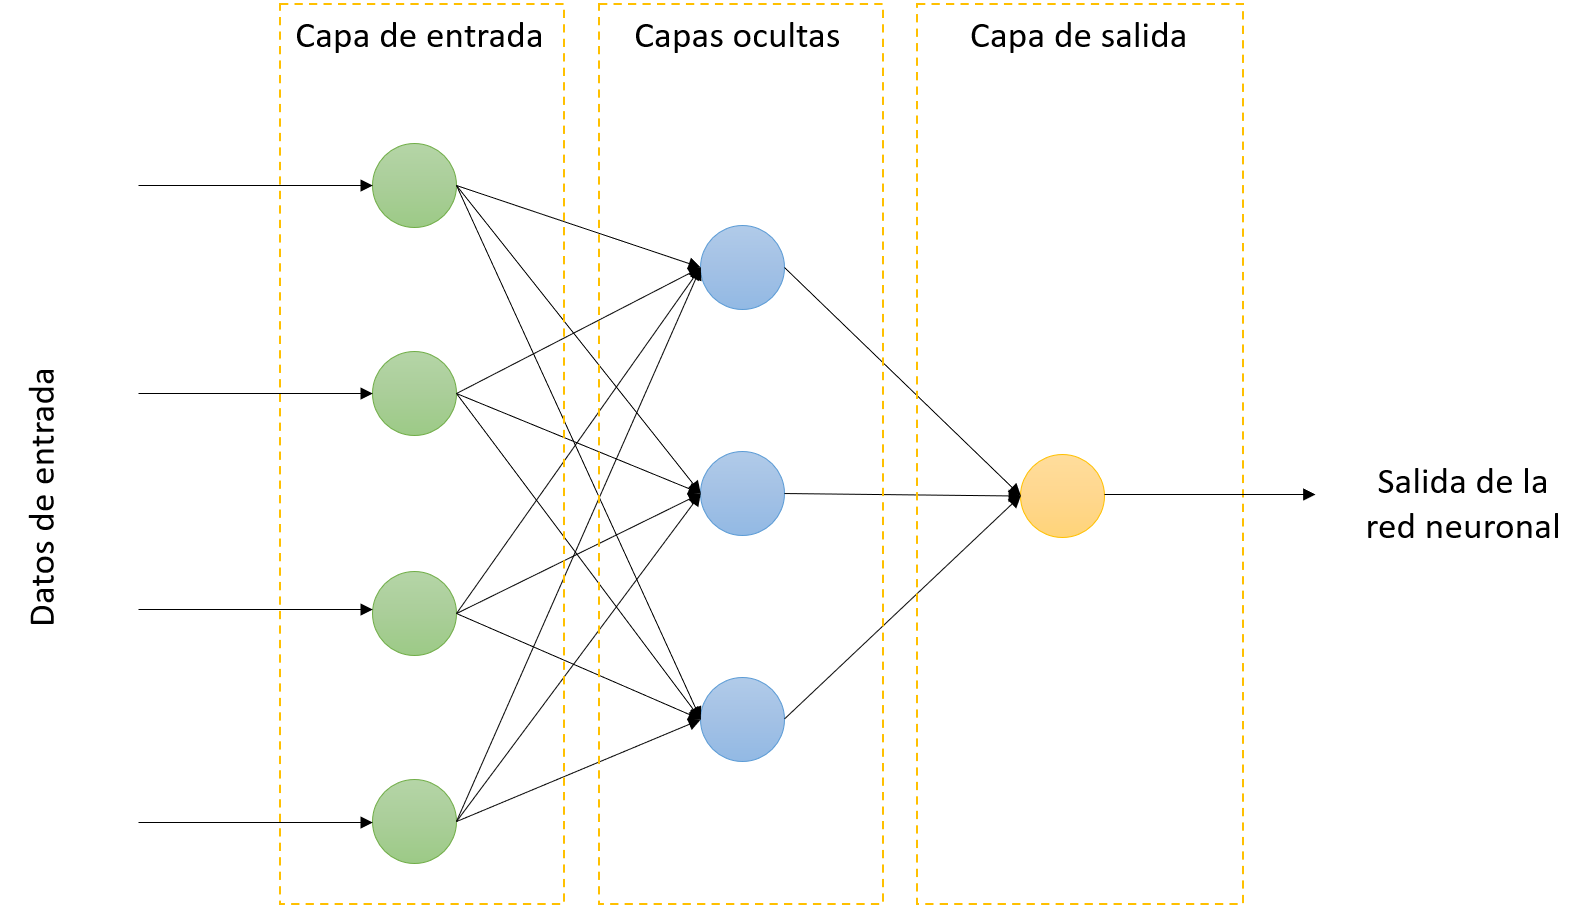
\includegraphics[width=0.8\textwidth]{Images/tutorial_ml_0215.png}
    \caption{Estructura típica de una red neuronal: incluye capa de entrada, capas ocultas y capa de salida.}
    \label{fig:estructura-red-neuronal}
\end{figure}
\textbf{ii. Inferencia por propagación hacia adelante} \\[3pt]
La propagación hacia adelante(\textit{forward propagation}) es el proceso por el que una red neuronal transforma los datos de entrada en predicciones o salidas, lo cual, si usamos tecnicismos, es el cálculo secuencial que mueve los datos desde la capa de entrada, a través de las capas ocultas y, finalmente, a la capa de salida. Durante este recorrido, los datos se transforman mediante conexiones ponderadas y funciones de activación, lo que permite a la red captar patrones complejos. \\
La importancia de la propagación hacia adelante radica en que es el mecanismo principal por el cual el modelo genera sus predicciones basadas en los parámetros que ha aprendido durante el entrenamiento que se le da. Sin este proceso, no sería posible evaluar cómo se comporta la red ante nuevos datos sin medir su desempeño. Además, la propagación hacia adelante es esencial para calcular la función de pérdida, que es la medición de los errores entre las predicciones y los valores reales. Esta información es usada posteriormente durante la retropropagación  para ajustar los pesos de la red y mejorar su precisión.
\begin{figure}[H]
    \centering
    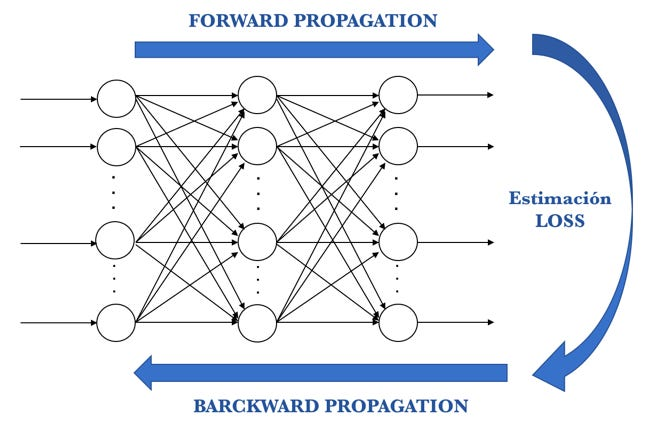
\includegraphics[width=0.6\textwidth]{Images/3eafe158-4126-48f0-ae70-65e707cc8988_668x427.jpg}
    \caption{Forward propagation and backward propagation}
    \label{fig:estructura-red-neuronal}
\end{figure}
\textbf{iii. Entrenamiento} \\[3pt]
El entrenamiento de una red neuronal es un proceso donde ajustamos pesos internos de la red con el fin de minimizar la diferencia entre las predicciones de la red y los valores reales esperados. Este proceso permite que la red aprenda a representar patrones presentes en los datos, generalizando su conocimiento para realizar predicciones sobre datos no vistos. El entrenamiento esta compuesto por dos fases principales: la evaluación del error, por medio de una \textbf{función de perdida}, y la \textbf{actualización de los pesos} usando el algoritmo de \textit{propagación hacia atrás} (\textit{backpropagation}).
\begin{itemize}
\item\textbf{1. Función de pérdida}:\newline
Es una función de pérdida cuantificada para saber qué tan bien o mal está funcionando una red. Calcula la diferencia entre la salida predicha por la red y el valor real esperado. El objetivo del entrenamiento es minimizar esta función de perdida mediante la actualización iterativa de los pesos. \newline Algunas funciones comunes son:
\begin{itemize}
    \item \textbf{Error cuadrático medio (MSE)}: Utilizada en tareas de regresión, se define como : $\mathcal{L}_{MSE} = \frac{1}{n} \sum_{i=1}^{n}(y_i - \hat{y}_i)^2$
    \item \textbf{Entropía cruzada}: Utilizada para clasificación, especialmente con salidas probabilísticas. Si se tiene una salida verdadera $y$ y una predicción $\hat{y}$, la pérdida es: $\mathcal{L}_{CE} = -\sum y \log(\hat{y})$
\end{itemize}

\item\textbf{2. Propagación hacia atrás (Backpropagation)}:\newline

\end{itemize}

\newpage
\thispagestyle{empty}
{\large \textbf{Fundamentos y justificación de GNNs}} \vspace{5pt}
\\
parte efrain

\newpage
\nocite{*}
\printbibliography
\end{document}



